% Clean beamerposter template — no external theme files, standard fonts.

\documentclass[final]{beamer}

\usepackage[T1]{fontenc}
\usepackage[utf8]{inputenc}
\usepackage{lmodern}
\usepackage[size=custom,width=122,height=91,scale=1.4]{beamerposter}
\usetheme{gemini}
\usepackage{graphicx}
\usepackage{amsmath,amssymb}
\usepackage{booktabs}
\usepackage{xcolor}
\usepackage{tikz}

% Suppress navigation bar
\setbeamertemplate{navigation symbols}{}

% Override gemini's Raleway font (not installed) with default sans-serif
\renewcommand{\Raleway}{}
\setbeamerfont{headline}{family=\sffamily}
\setbeamerfont{block title}{size=\large,series=\bfseries,family=\sffamily}

% ==================
% Kentucky blue colors
% ==================
\definecolor{ukblue}{RGB}{0,51,160}
\definecolor{ukbluedark}{RGB}{0,33,105}
\definecolor{blockbg}{RGB}{245,247,252}

\setbeamercolor{background canvas}{bg=white}
\setbeamercolor{headline}{bg=ukbluedark,fg=white}
\setbeamercolor{headline rule}{bg=ukblue}
\setbeamercolor{title in headline}{fg=white}
\setbeamercolor{author in headline}{fg=white}
\setbeamercolor{institute in headline}{fg=white}
\setbeamercolor{block title}{bg=ukblue,fg=white}
\setbeamercolor{block separator}{bg=ukblue}
\setbeamercolor{block body}{bg=blockbg,fg=black}
\setbeamercolor{footline}{bg=ukbluedark,fg=white}
\setbeamercolor{structure}{fg=ukblue}

% ==================
% Headline (title banner)
% ==================
% Headline: two-line title + authors on UK blue banner
\setbeamertemplate{headline}{
  \begin{beamercolorbox}[wd=\paperwidth,center,leftskip=5ex,rightskip=5ex]{headline}
    \vskip5ex
    {\sffamily\fontsize{70}{82}\selectfont\bfseries\color{white}
      Message-Passing Graph Neural Network as a Surrogate\par}
    \vskip1ex
    {\sffamily\fontsize{70}{82}\selectfont\bfseries\color{white}
      for Variable-Length 1D Finite Element Bead Chain Simulations\par}
    \vskip3ex
    {\sffamily\fontsize{40}{48}\selectfont\color{white}\insertauthor\par}
    \vskip5ex
  \end{beamercolorbox}
}

% ==================
% Block templates
% ==================
\setbeamertemplate{block begin}{
  \begin{beamercolorbox}[wd=\textwidth,leftskip=1ex,rightskip=1ex]{block title}
    \vskip0.6ex
    {\fontsize{26}{30}\selectfont\bfseries\color{white}\insertblocktitle\par}
    \vskip0.6ex
  \end{beamercolorbox}
  \vskip-1pt
  \begin{beamercolorbox}[wd=\textwidth,leftskip=1ex,rightskip=1ex,vmode]{block body}
  \vskip1ex
}
\setbeamertemplate{block end}{
  \vskip1ex
  \end{beamercolorbox}
  \vspace{1.5ex}
}

% ==================
% Footer (gemini already defines \footercontent)
% ==================
\setbeamertemplate{footline}{
  \begin{beamercolorbox}[wd=\paperwidth,ht=5ex,dp=2ex,leftskip=3ex,rightskip=3ex]{footline}
    \vfill
    {\sffamily\fontsize{28}{34}\selectfont\color{white}\insertfootercontent}
    \vfill
  \end{beamercolorbox}
}

% ==================
% Column lengths
% ==================
\newlength{\sepwidth}
\newlength{\colwidth}
\setlength{\sepwidth}{0.025\paperwidth}
\setlength{\colwidth}{0.3\paperwidth}
\newcommand{\separatorcolumn}{\begin{column}{\sepwidth}\end{column}}

% ==================
% Title
% ==================
\title{Message-Passing Graph Neural Network as a Surrogate for Variable-Length 1D Finite Element Bead Chain Simulations}
\author{Grey L.~Goodwin \quad\textbf{\textperiodcentered}\quad Daniel L.~Lau, PhD.}
\footercontent{Department of Electrical and Computer Engineering, University of Kentucky \hfill grey.goodwin@uky.edu}

\begin{document}
\begin{frame}[t]
\begin{columns}[t]
\separatorcolumn

% =============== COLUMN 1 ===============
\begin{column}{\colwidth}

  \begin{block}{Abstract}
    Finite element analysis (FEA) of a flexible bead chain requires
    thousands of small, localized force and integration computations per
    simulated second. We train a graph neural network (GNN) to predict the
    per-timestep physics of a 1D bead chain with tapered mass, using
    randomly sampled single-step training data instead of recorded
    simulations. A key finding was that even a well-designed model will
    fail without the correct training data. An initial shared MLP achieved
    accurate predictions on a fixed 16-bead chain but could not generalize
    to other lengths. We restructure the surrogate as a true
    message-passing GNN with separate node/edge encoders, learned messages
    per rod, and ghost masking for endpoints. Because all weights are
    shared, one trained model handles chains of any length. We train on 1M
    volume-sampled scenarios from chains of 8--32 beads and evaluate on
    chain lengths, orientations, and velocities never seen during training.
  \end{block}

  \begin{block}{Problem Setup}
    A whip is modeled as a 1D chain of $N$ tapered mass nodes connected
    by $N-1$ spring rods, anchored at one end. Each free bead experiences
    gravity, Hookean spring forces, rod-axis damping, and velocity drag.
    Time integration uses symplectic Euler:
    \begin{equation}
        \mathbf{v}_i^{n+1} = \mathbf{v}_i^n + \Delta t \, \mathbf{a}(\mathbf{x}^n)
    \end{equation}
    \begin{equation}
        \mathbf{x}_i^{n+1} = \mathbf{x}_i^n + \Delta t \, \mathbf{v}_i^{n+1}
    \end{equation}
    The force on bead $i$ depends only on its state and those of its
    immediate neighbors. This locality is why we use a 1-hop graph
    architecture.
  \end{block}

  \begin{block}{MPGNN Architecture}
    \begin{itemize}
      \item \textbf{Node encoder} $(4 \to 64)$: $[v_x, v_y, m, \text{fixed}]$
      \item \textbf{Edge encoder} $(6 \to 64)$: shared left/right, relative features
      \item \textbf{Message MLP} $(64 \to 64)$: per-edge learned message
      \item \textbf{Ghost mask}: zero messages from absent neighbors
      \item \textbf{Node update MLP} $(192 \to 64)$: fuses self + messages
      \item \textbf{Output head} $(64 \to 4)$: change in state
    \end{itemize}
    80{,}324 parameters, shared across all beads, independent of chain
    length.
  \end{block}

\end{column}

\separatorcolumn

% =============== COLUMN 2 ===============
\begin{column}{\colwidth}

  \begin{block}{Data Pipeline: Volume-Sampled Per-Bead Physics}
    Rather than recording trajectories, we sample random single-step
    scenarios uniformly across the reachable state space. Each sample is
    one bead at one instant plus the exact physics result one timestep later.

    \begin{figure}
      \centering
      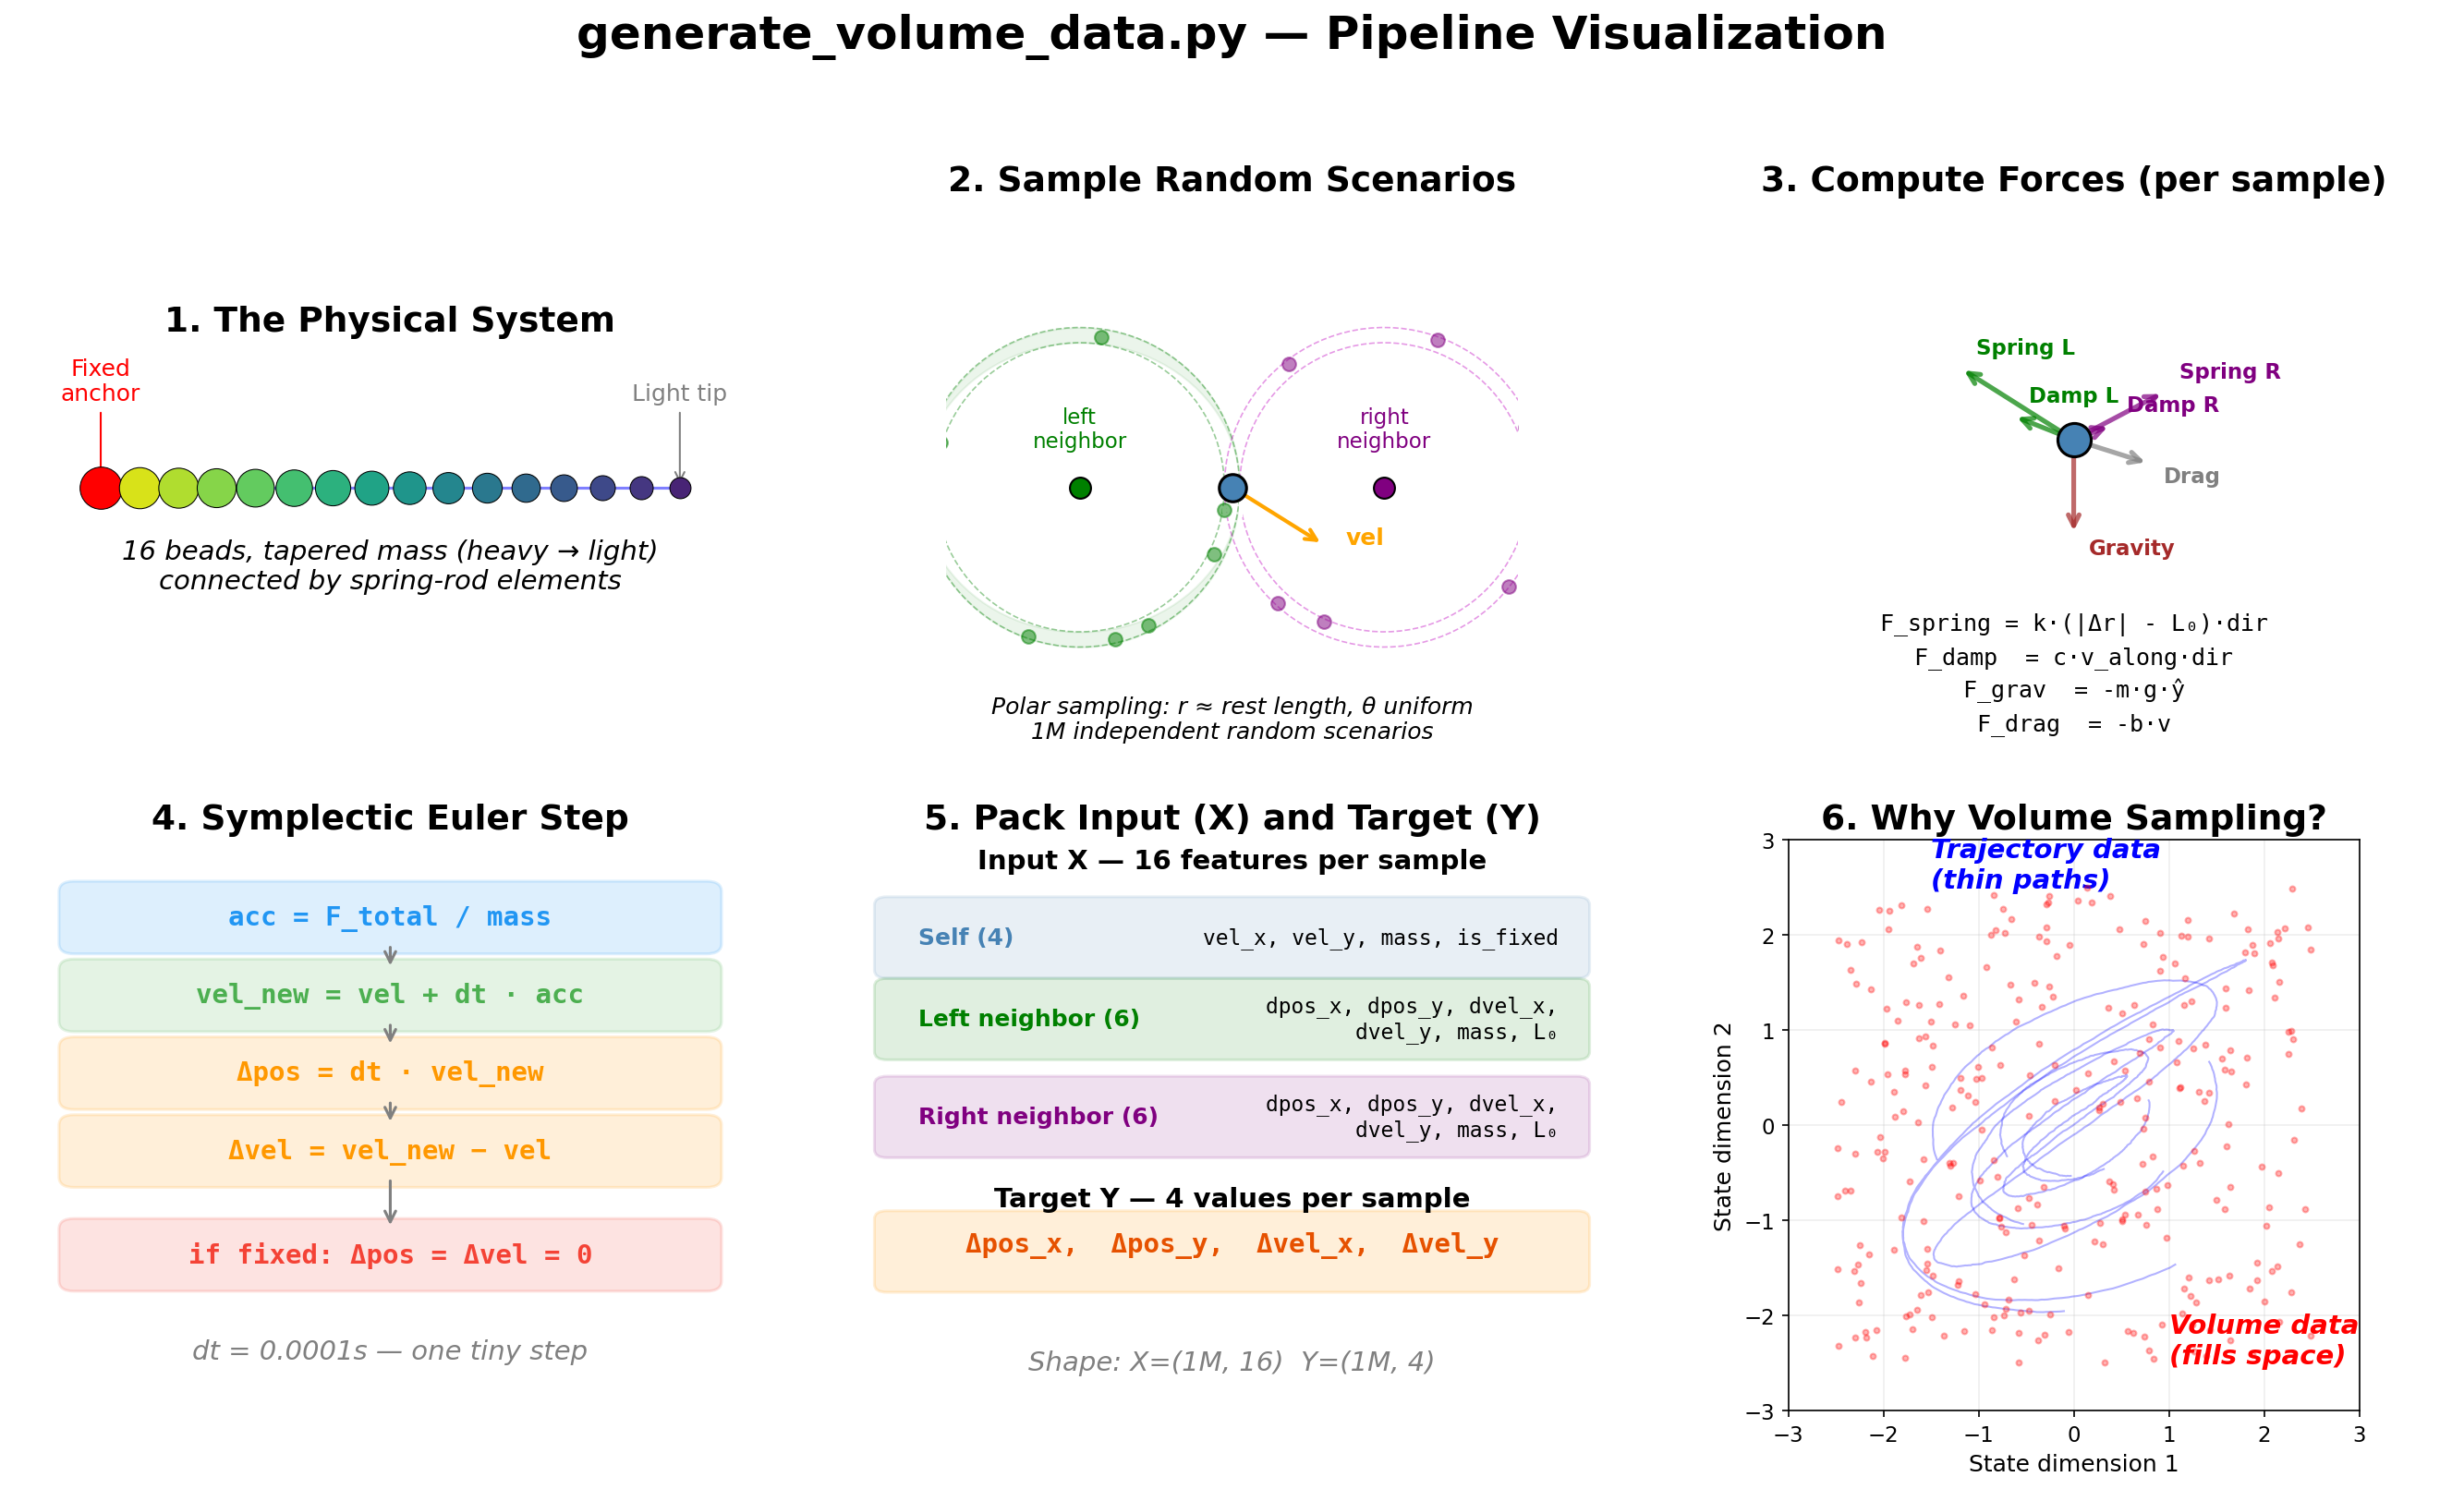
\includegraphics[width=\textwidth]{pipeline_visualization.png}
    \end{figure}

    (1)~Tapered chain with rods. (2)~Neighbor positions drawn in polar
    coordinates. (3)~Forces computed on central bead. (4)~Symplectic
    Euler step. (5)~Inputs (16 features) and targets (4 deltas) packed.
    (6)~Volume sampling covers state space uniformly.
  \end{block}

  \begin{block}{Why Volume Sampling?}
    Trajectory data traces thin curves through state space; small rollout
    errors push the simulation off those curves into regions without
    training coverage. Volume sampling gives the model coverage across the full state space,
    not just along specific trajectories.
    Combined with randomized chain lengths ($N \in [8, 32]$) and taper
    ratios ($r \in [1, 10]$), the training data is not tied to any
    specific chain configuration.
  \end{block}

\end{column}

\separatorcolumn

% =============== COLUMN 3 ===============
\begin{column}{\colwidth}

  \begin{block}{Training Convergence}
    \begin{figure}
      \centering
      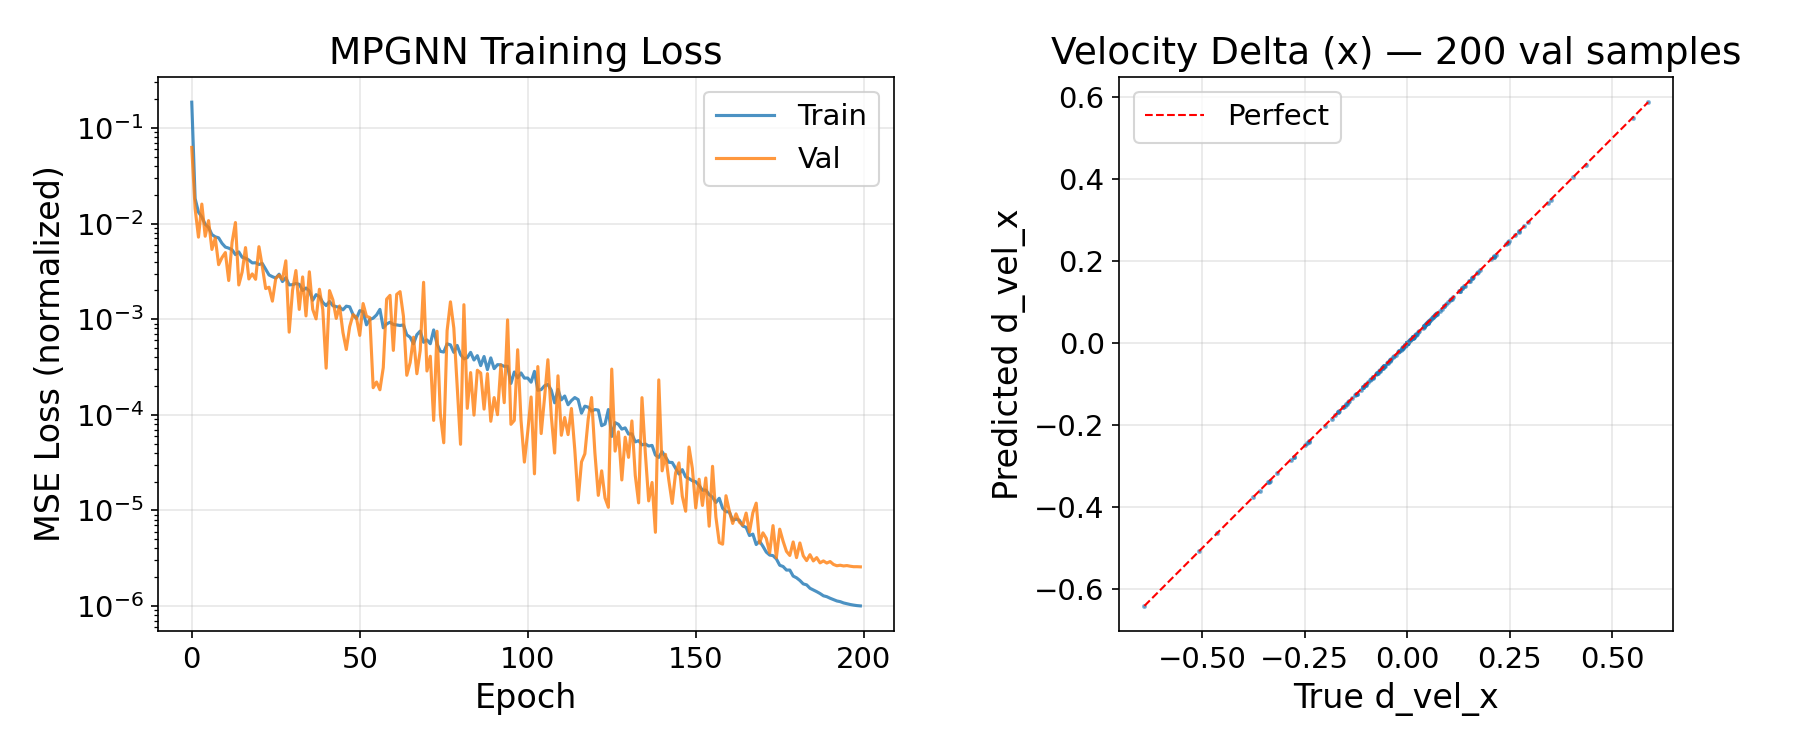
\includegraphics[width=\textwidth]{mpgnn_training.png}
    \end{figure}
    Train/validation MSE loss over 200 epochs (left) and predicted
    vs.\ true $\Delta v_x$ on validation samples (right). Predictions match the ground truth closely.
  \end{block}

  \begin{block}{Generalization Across Chain Lengths}
    \begin{figure}
      \centering
      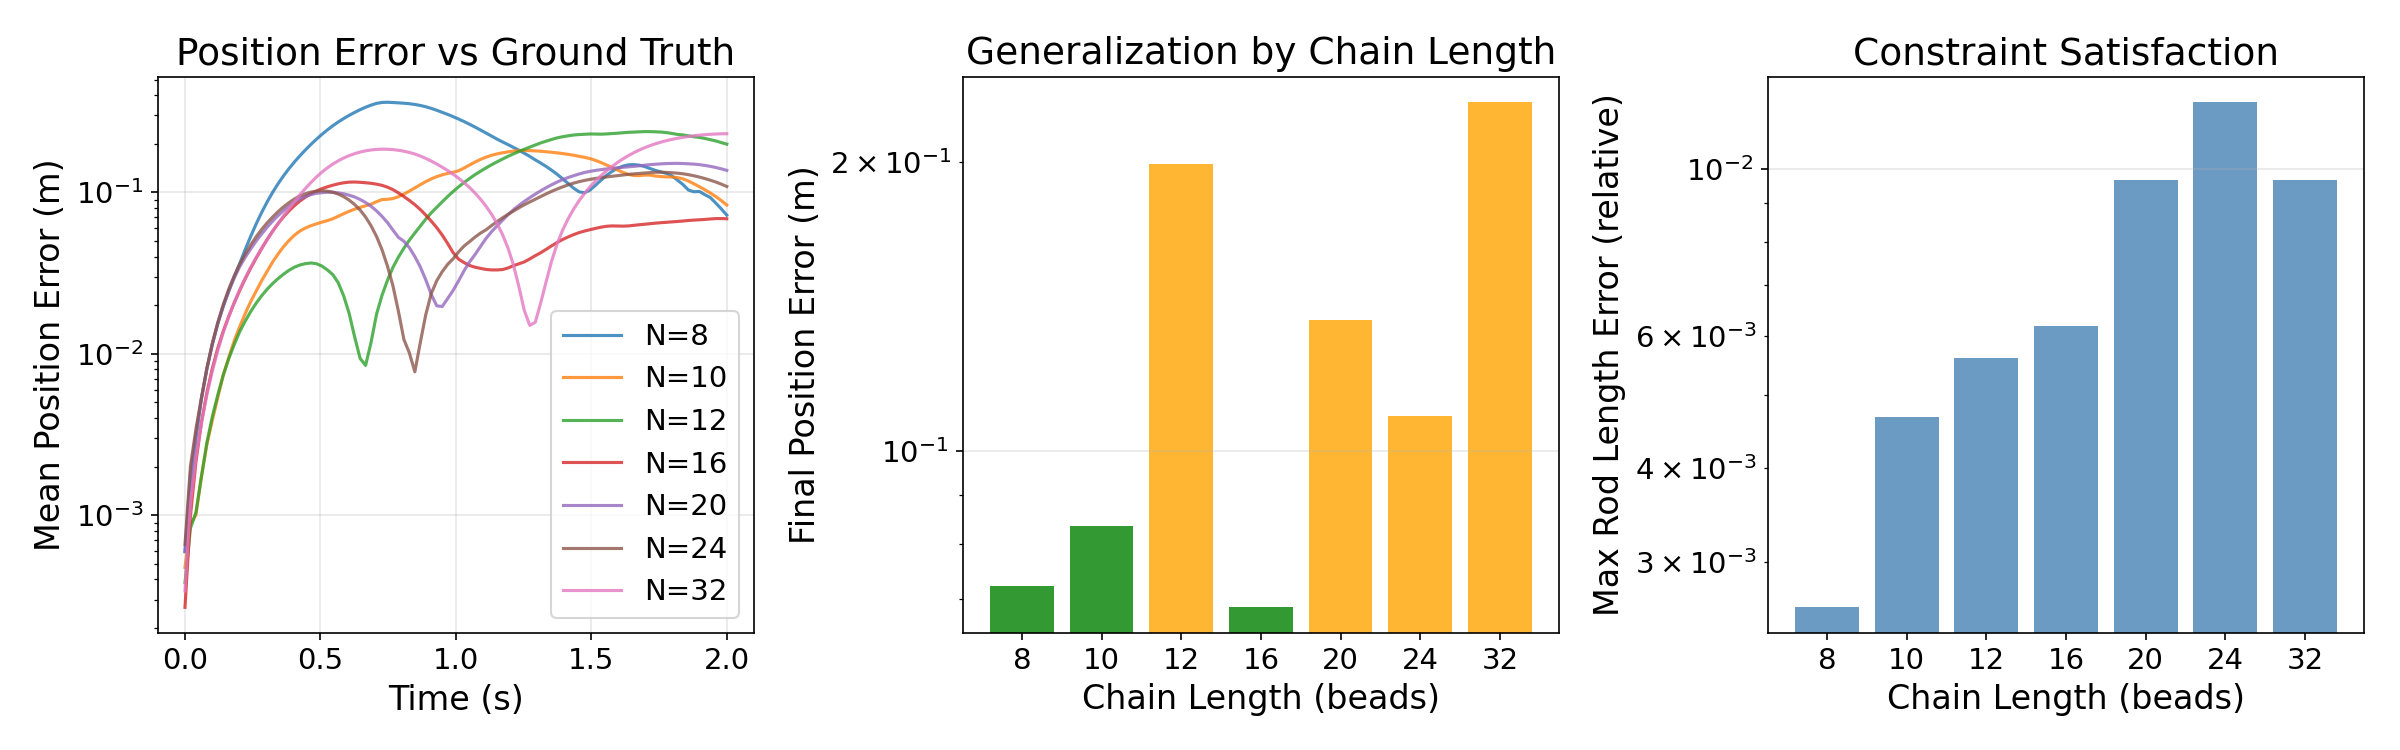
\includegraphics[width=\textwidth]{mpgnn_variable_eval.png}
    \end{figure}
    Trained MPGNN evaluated on chains of
    $N \in \{8, 10, 12, 16, 20, 24, 32\}$ via full rollouts. Short and
    medium chains track closely; longer chains accumulate more drift.
  \end{block}

  \begin{block}{Conclusion and Future Work}
    Replacing a fixed-size MLP with a weight-shared message-passing GNN
    lets one trained model simulate bead chains of any length.
    Separate node/edge encoders, per-rod messages, and ghost masking
    make this possible. Volume sampling provides the training coverage
    needed for stable rollouts.

    \textbf{Future work:} rollout training to reduce drift and deeper
    message-passing with broader training data.
  \end{block}

\end{column}

\separatorcolumn
\end{columns}
\end{frame}
\end{document}
